\chapter{Heterogeneous Knowledge Graph Construction}
\label{chap:kg}

\section{Motivation: Why a Heterogeneous Graph?}
\label{sec:kg_motivation}

The cleaned case JSONs from Chapter~\ref{chap:pipeline} carry typed entities, rhetorical-role-segmented text, and outcome labels. A flat representation --- concatenate preamble, facts, and arguments and feed the blob to a transformer --- has two costs. First, it discards typed structure already present in the data: a court, a statute, a provision, and a party are four different kinds of object with different evidential value, and flattening forces the model to re-learn that. Second, it has no way to exchange information \emph{between} cases that share legally meaningful objects. When Case~A and Case~B both cite IPC~498A, the flat view sees the string twice; the graph view attaches both cases to the same \textsc{Statute} node and, through one round of message passing, lets A's representation influence B's.

A heterogeneous graph captures both properties: \emph{heterogeneous} because node types carry different features and relational semantics, and a \emph{graph} because legally important relationships are relational (a case \emph{is heard in} a court, an argument block \emph{cites} a statute, a provision \emph{belongs to} a statute).

\section{Graph Schema}
\label{sec:graph_schema}

The graph is a \textbf{full-star global graph}: every case is a local star of text and entity nodes anchored on a \textsc{Case} node, and a selected set of entity types are \emph{shared} across cases so that stars of different cases are stitched into one connected component.

\subsection{Node Types}

The reasoning-focused graph keeps \textbf{17 node types} in three categories:

\begin{sloppypar}
\begin{itemize}
  \item \textbf{Case node.} A single \textsc{Case} node per case, with attributes for outcome label, bucket, filing/decision dates (for temporal gating), and metadata.
  \item \textbf{Text nodes.} Six types --- \textsc{Preamble}, \textsc{Facts}, \textsc{Arguments}, \textsc{Petitioner\_Arguments}, \textsc{Respondent\_Arguments}, \textsc{Other\_Lawyer\_Arguments} --- each carrying a \texttt{bge-m3} embedding of the cleaned, leakage-filtered span (Section~\ref{sec:text_features}).
  \item \textbf{Entity nodes.} Ten types: \textsc{Petitioner}, \textsc{Respondent}, \textsc{Petitioner\_Lawyer}, \textsc{Defence\_Lawyer}, \textsc{Lawyer}, \textsc{Court}, \textsc{Judge}, \textsc{Statute}, \textsc{Provision}, \textsc{Precedent}.
\end{itemize}
\end{sloppypar}

The auxiliary NER types (\textsc{Org}, \textsc{GPE}, \textsc{Date}, \textsc{Case\_Number}) are removed: they carry little predictive signal and would introduce weak, noisy edges that dilute message passing.

\subsection{Cross-Case Sharing}

Whether two cases share a node or each hold a private copy determines whether a GNN can use that node as a cross-case conduit:

\begin{itemize}
  \item \textbf{Shared across cases}: \textsc{Statute}, \textsc{Provision}, \textsc{Precedent} --- the \emph{law itself}. Citing IPC~420 in one case and IPC~420 in another is the same object; sharing is what lets the GNN propagate along the citation.
  \item \textbf{Local to each case}: everything else, including \textsc{Court}, \textsc{Judge}, and all \textsc{Lawyer} variants --- \emph{identity proxies}. Sharing them would let the GNN recover judge- or bench-level win/loss bias as a free shortcut. Keeping them local makes the model reason about the law, not the docket.
\end{itemize}

\subsection{Edge Types}

\begin{sloppypar}
Core typed edges: \path{case--has_preamble/has_facts/has_arguments--*text*} attach text nodes; \path{case--has_petitioner_arguments/has_respondent_arguments/has_other_lawyer_arguments--*text*} attach party-specific argument blocks; \path{case--has_petitioner/has_respondent--*party*}, \path{case--heard_in--court}, \path{case--decided_by_bench--judge}, and the \path{has_*_lawyer} edges attach participants. The citation backbone is \path{arguments--cites_statute--statute}, \path{arguments--cites_provision--provision}, \path{arguments--cites_precedent--precedent} --- attached to the \textsc{Arguments} node so citations sit in their legal-discourse context --- together with \path{provision--belongs_to_statute--statute}. Counsel nodes are linked to their argument blocks via \path{citation} edges, and parties to their own blocks via \path{is_party_in_arguments}. All edges are added with reverse counterparts and the final graph is passed through \texttt{to\_undirected} so HGT's typed message passing flows both ways.
\end{sloppypar}

\paragraph{Intentionally removed shortcut edges.} An earlier schema added edges letting entities bypass the arguments node --- \texttt{statute--used\_in\_arguments}, \texttt{judge--presided\_arguments}, party edges to the shared \textsc{Arguments} node. These are now forbidden: they created short paths from identity proxies to the case representation with little reasoning value but much spurious correlation.

\subsection{Attributes}

Every \textsc{Case} node carries a binary outcome label ($+1$ win, $-1$ loss) plus bucket and dates. Text nodes carry the raw span (for inspection only) and its embedding. Entity nodes carry canonical names and canonicalisation metadata. Edges are attributed with their relation type, which HGT uses to index per-relation parameters.

\subsection{Visualising the Graph Structure}
\label{sec:graph_visualizations}

Figure~\ref{fig:single_case_graph} shows the local star surrounding a single \textsc{Case} node. The Arguments node branches out to Statutes, Provisions, and Precedents. Citation edges maintain a strict chronological hierarchy: a case forms a citation edge to a Precedent only when $\text{precedent\_year} < \text{case\_year}$, and to a Statute only when $\text{statute\_year} \leq \text{case\_year}$, ensuring older cases cannot structurally link forward in time.

\begin{figure}[htbp]
    \centering
    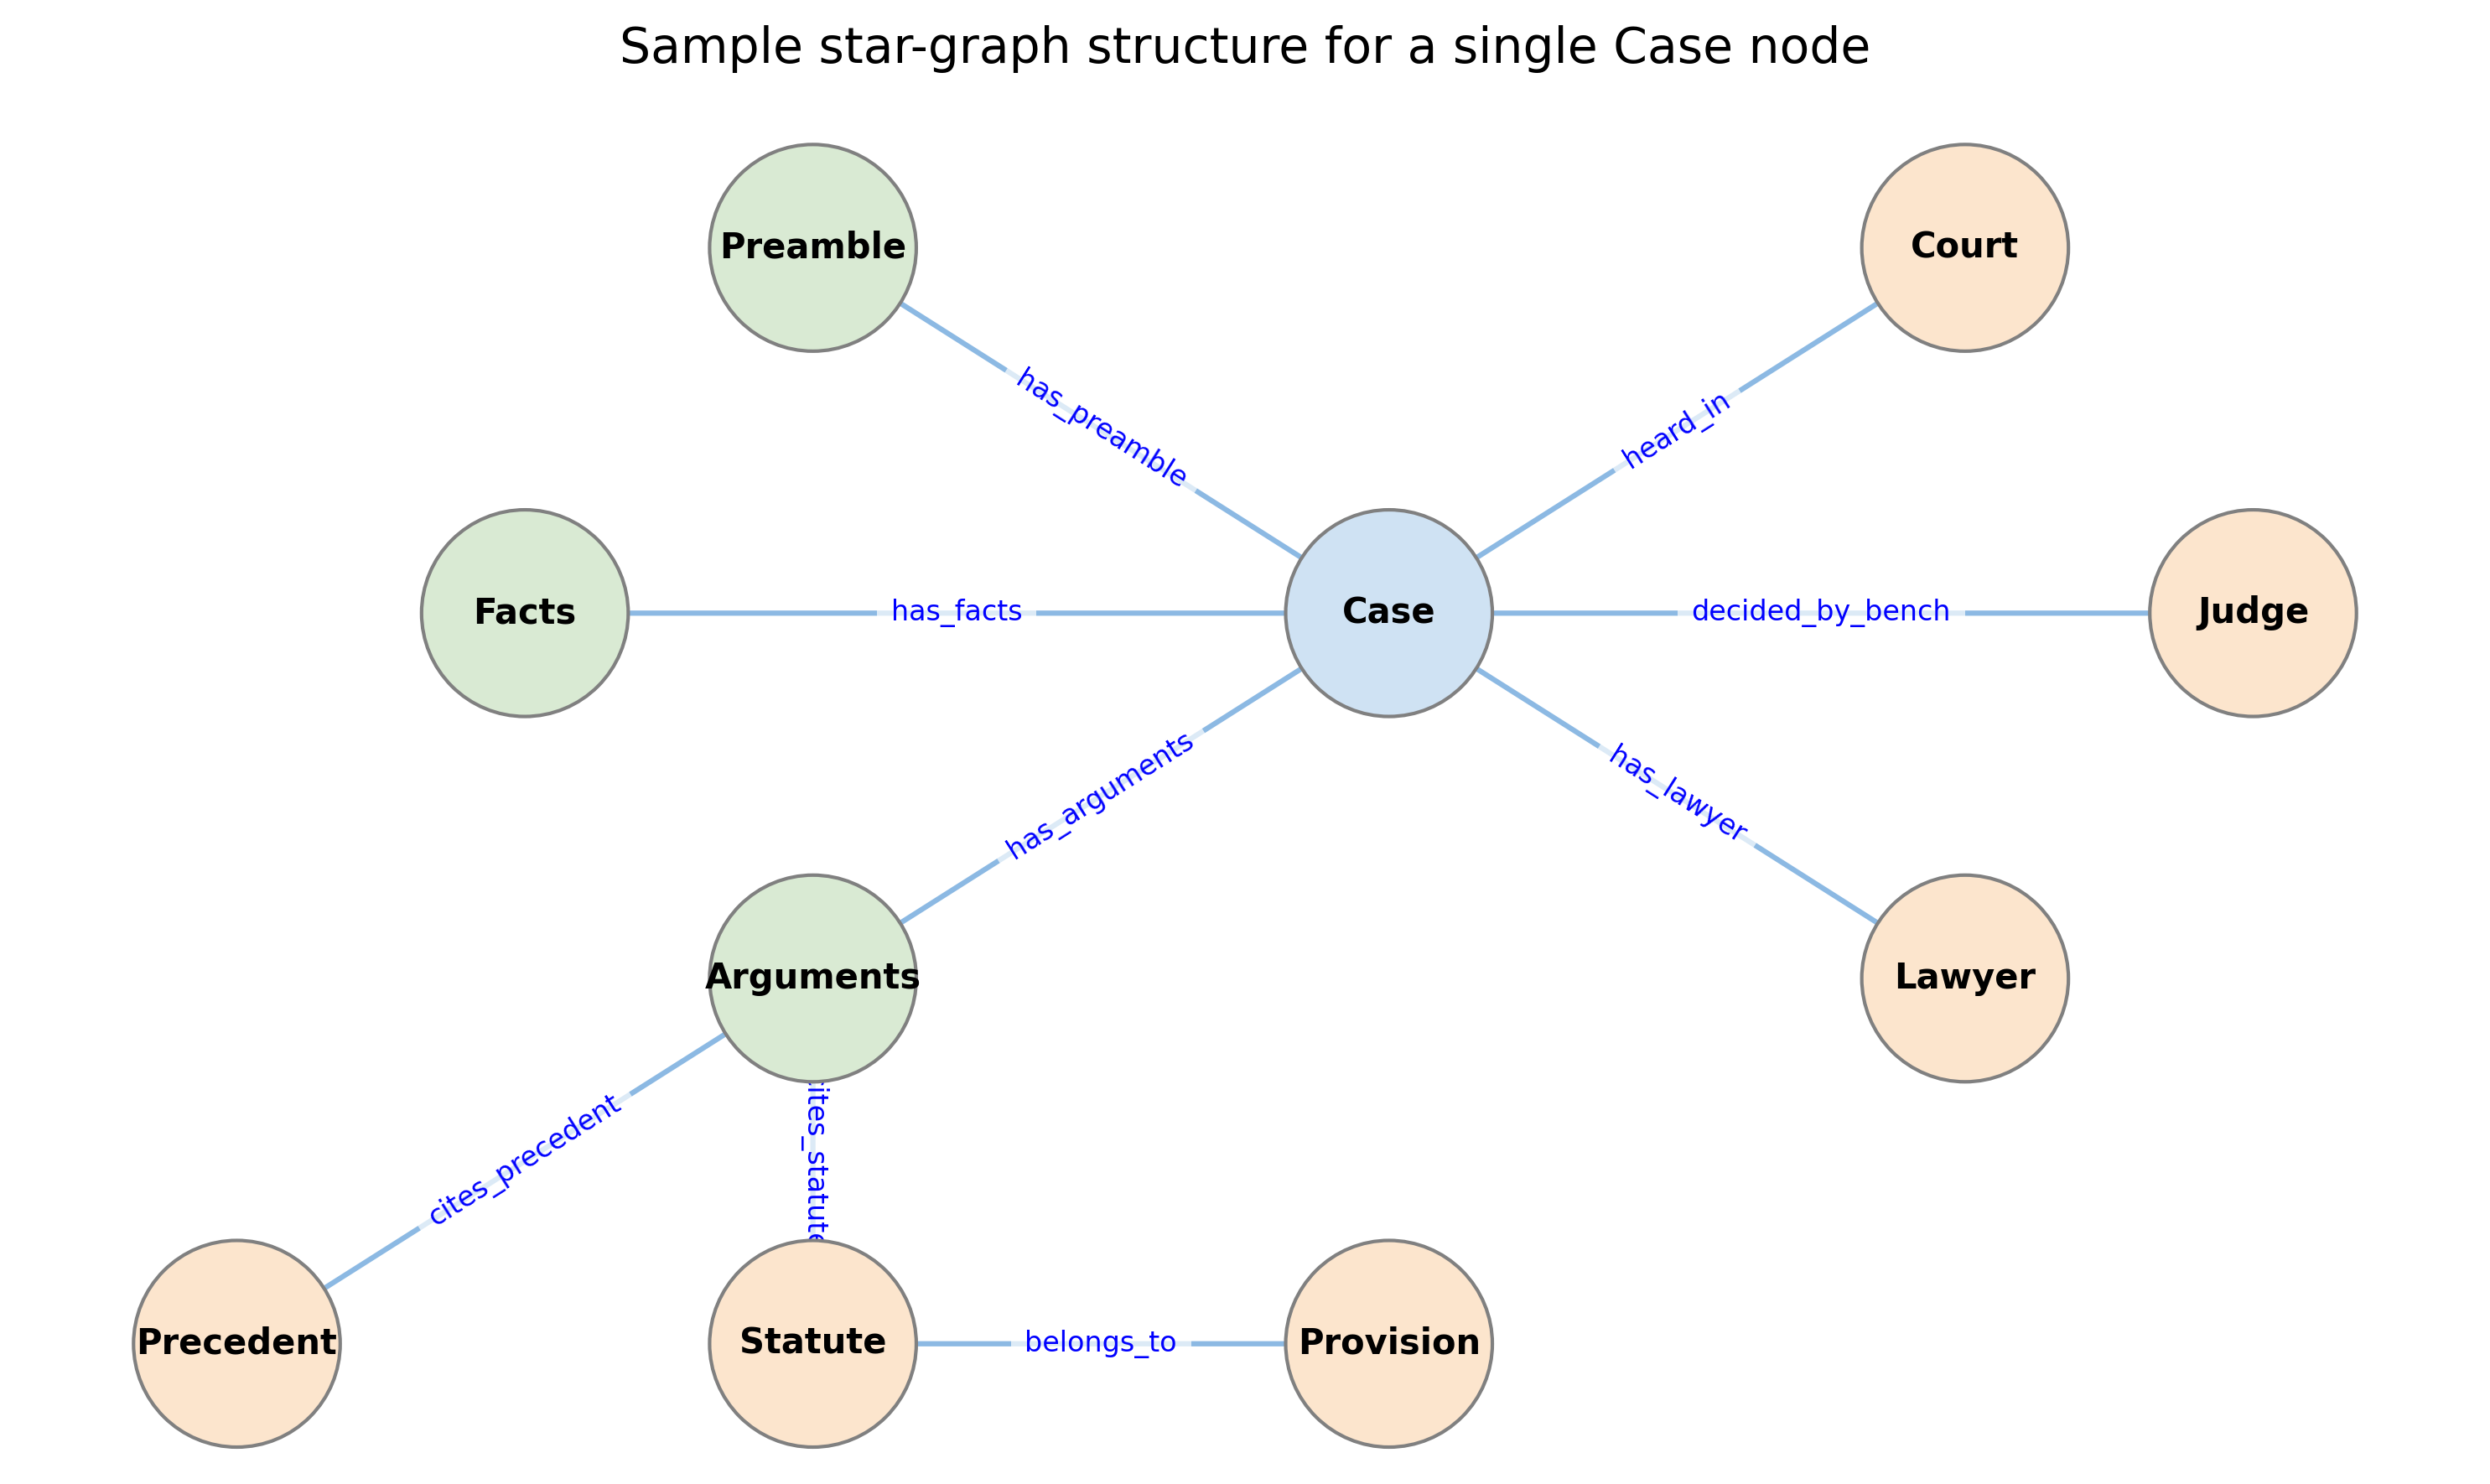
\includegraphics[width=\textwidth]{figures/single_case_graph.png}
    \caption{Star-graph structure for a single Case node. Text blocks and entity nodes surround the case; the Arguments node branches out to shared legal concepts.}
    \label{fig:single_case_graph}
\end{figure}

Figure~\ref{fig:cross_case_graph} shows cross-case sharing. Courts and Judges are private; Statutes, Provisions, and Precedents are shared, acting as cross-case conduits that let the GNN reason without observing outcome proxies.

\begin{figure}[htbp]
    \centering
    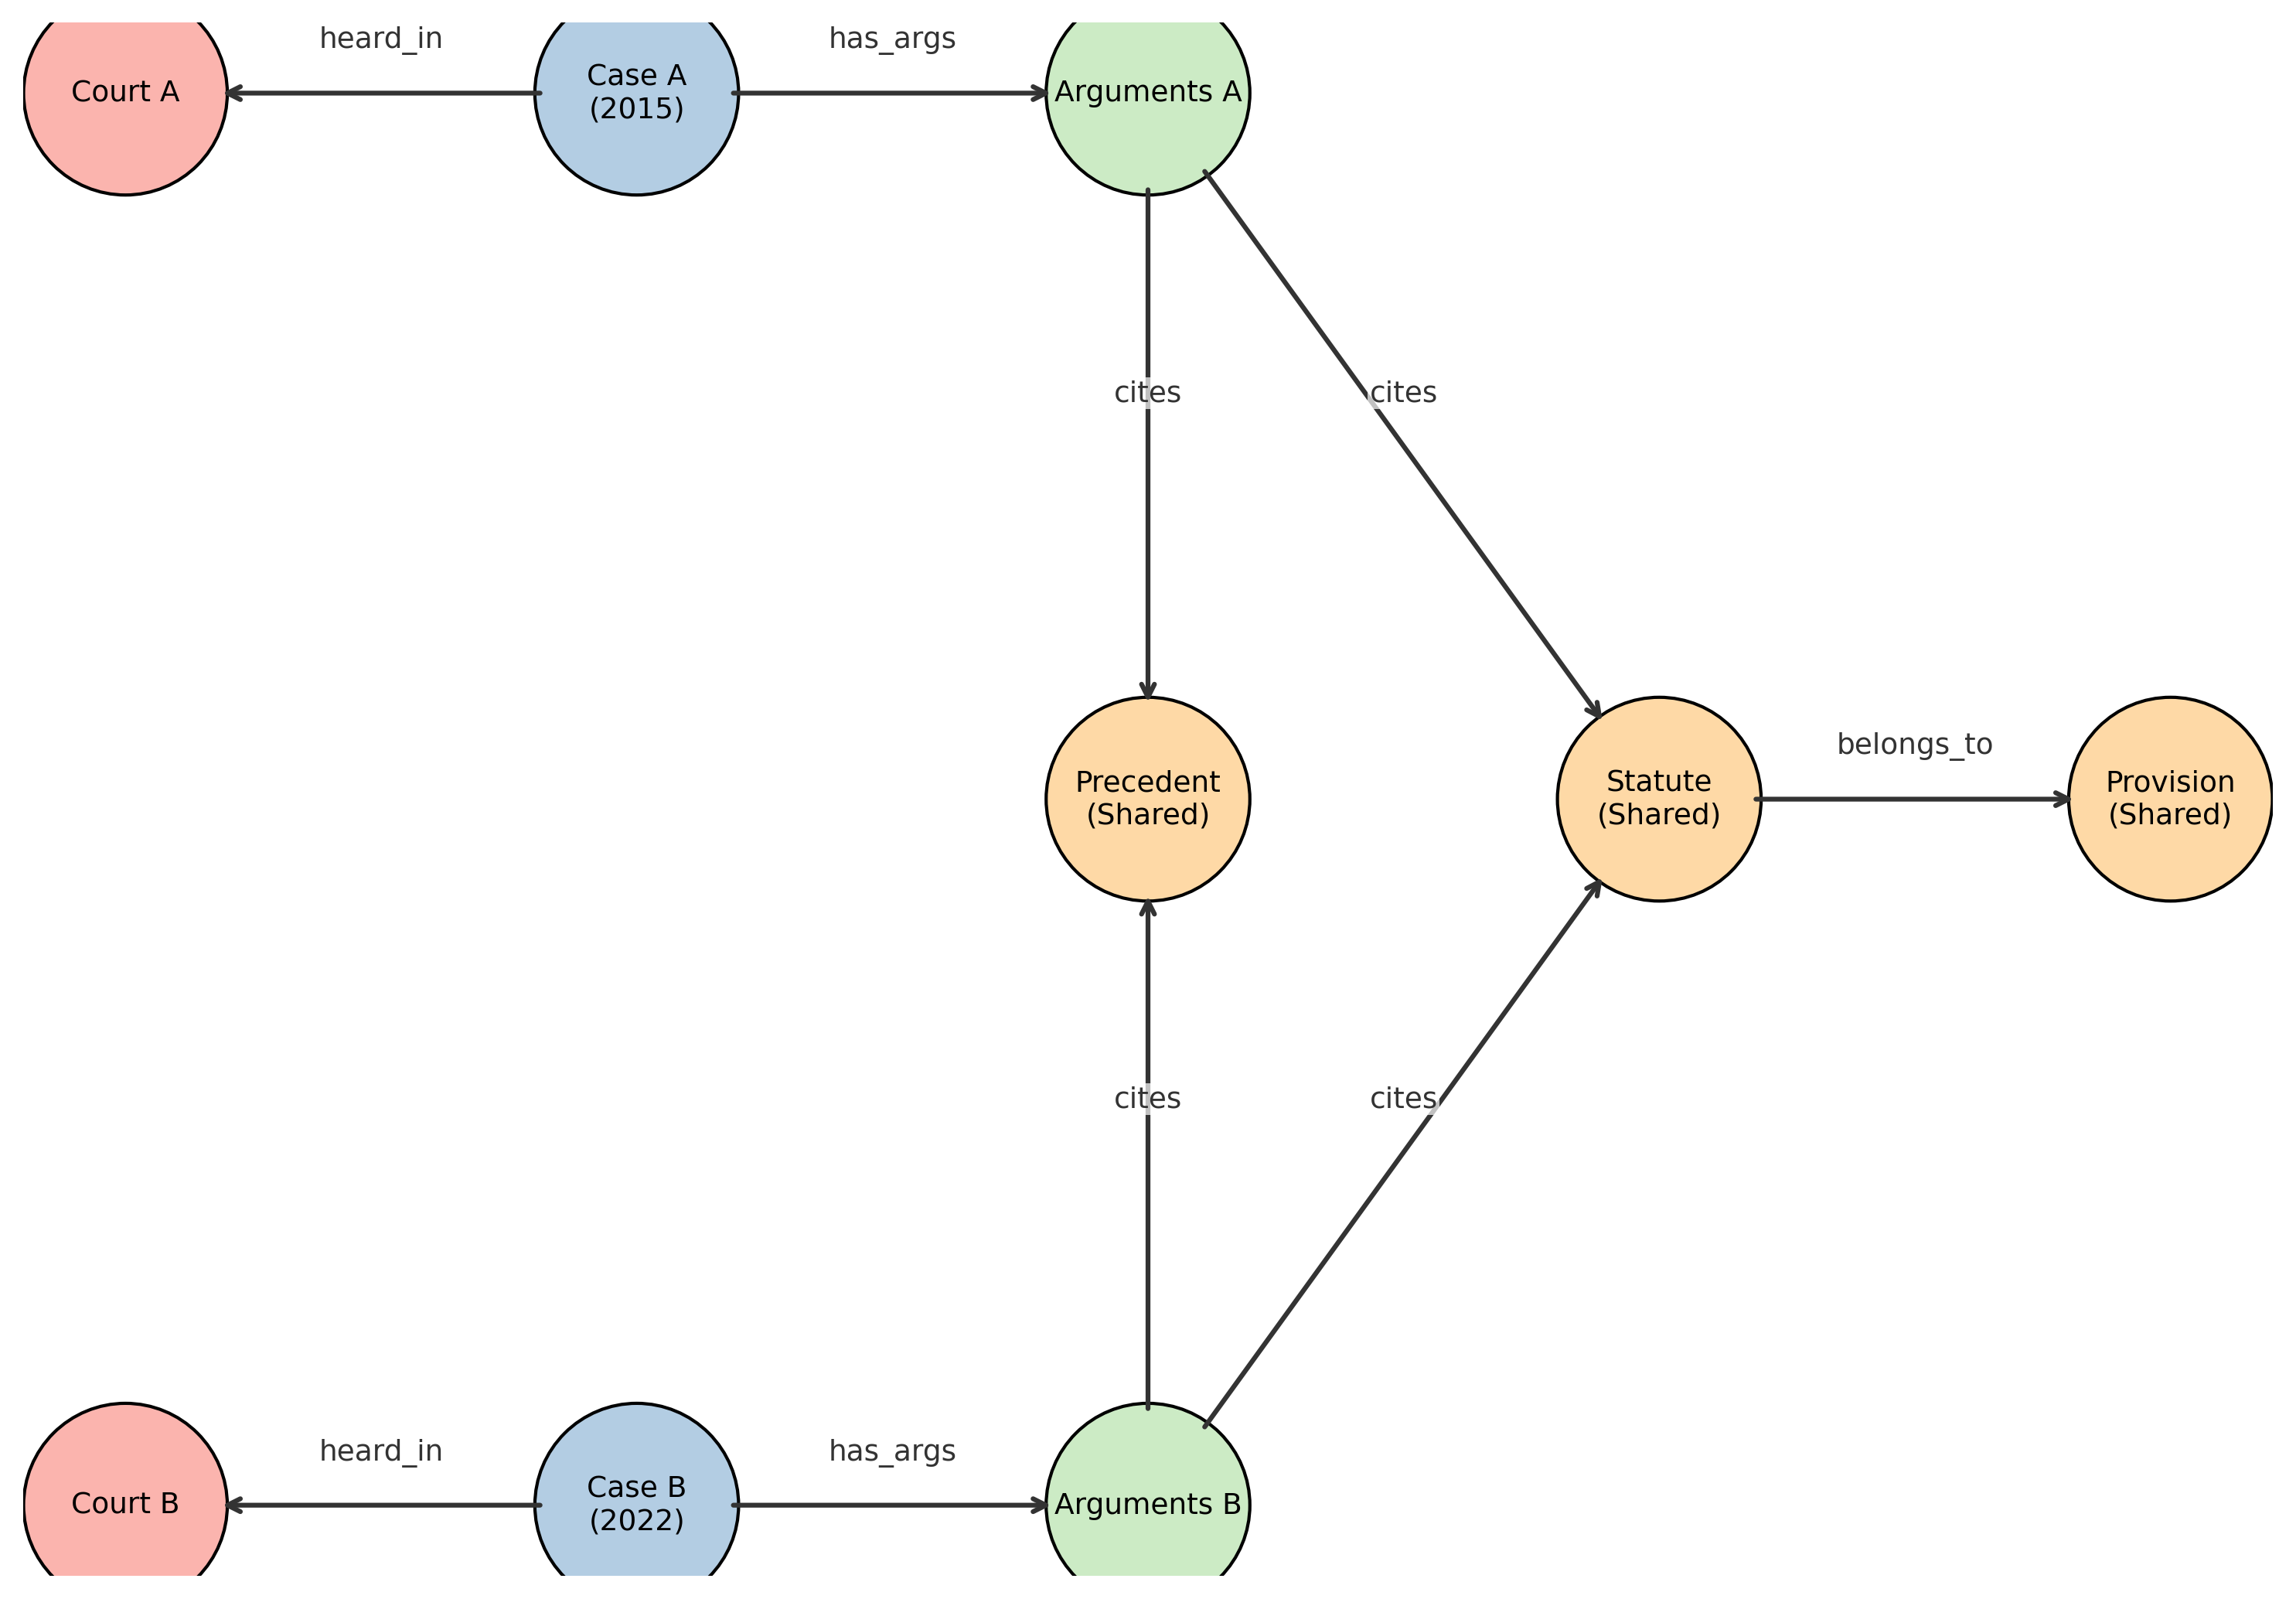
\includegraphics[width=\textwidth]{figures/schema_cross_case.png}
    \caption{Cross-connection of cases via shared nodes. Identity entities remain local; statutes and precedents act as legally sound cross-case conduits.}
    \label{fig:cross_case_graph}
\end{figure}

\section{Leakage Prevention Strategy}
\label{sec:leakage_prevention}

LJP has a notorious failure mode: models that appear to predict the outcome are actually \emph{reading} it. The pipeline defends against this at five points:

\begin{sloppypar}
\paragraph{1.\ Field-level removal.} Cleaning drops \path{FORBIDDEN_TOP_LEVEL_FIELDS} --- \texttt{case\_outcome\_label}, \texttt{case\_outcome\_score}, \texttt{llm\_case\_outcome}, \texttt{decision\_text}, \texttt{rpc\_texts}, \texttt{short\_explanation}, \texttt{raw\_model\_response} --- plus the \texttt{raw\_result.summary.decision} block.

\paragraph{2.\ Rhetorical-role filtering.} Annotations whose labels intersect \{\textsc{RPC}, \textsc{RLC}\} or whose label strings contain \texttt{decision}, \texttt{disposition}, \texttt{operative}, \texttt{order}, or \texttt{rpc} are removed before text nodes are built. Because \textsc{RPC} is where the court pronounces the result, this is the single most important filter.

\paragraph{3.\ Phrase-level masking.} A list \texttt{DEFAULT\_LEAKAGE\_PHRASES} (\emph{``petition stands disposed of''}, \emph{``appeal is allowed''}, \emph{``set aside''}, \emph{``quashed''}, \dots) is compiled to case-insensitive regex and applied across every retained field. Matches are logged and replaced with a \texttt{[LEAKAGE\_MASK]} token, catching residual decision fragments embedded in \textsc{Facts} or \textsc{Arguments} sentences the RR filter missed.

\paragraph{4.\ Temporal gating on shared entities.} A precedent citation edge is added only when $\text{precedent\_year} < \text{case\_year}$; a statute citation edge only when $\text{statute\_year} \leq \text{case\_year}$.

\paragraph{5.\ Audit trail.} Every case carries a \texttt{leakage\_audit} recording dropped fields, removed annotations, and every phrase-level mask, stored with the graph cache so leakage claims can be \emph{disproved}, not merely argued against.
\end{sloppypar}

The combined effect is that the text a GNN layer sees through text-node features is a pre-decision representation of the dispute --- who the parties are, what happened, what each side argued, what law they cited --- with the decision systematically withheld.

\section{Text Embedding and Feature Extraction}
\label{sec:text_features}

\subsection{The \texttt{bge-m3} Text Encoder}

All text nodes are featurised with \path{BAAI/bge-m3}, a multilingual sentence-transformer with a $1024$-dim output. Two reasons: (i) Indian legal text mixes English with Hindi and regional-language transliterations, Latin-script legal abbreviations, and citation fragments, where \texttt{bge-m3}'s multilingual training handles noise better than English-only encoders; and (ii) the model is strong in retrieval settings, aligning with the graph's use of embeddings as comparison features.

The encoder runs with \texttt{batch\_size=16}, \texttt{max\_length=512}, on GPU, in multi-process mode across CUDA devices. For spans exceeding the $512$-token window, the encoder splits them into overlapping, sentence-boundary-aligned chunks, encodes each independently, and mean-pools --- preserving a consistent $1024$-dim representation per node regardless of length. Embeddings are cached per namespace with a deterministic hash of ids, texts, and encoder configuration; changing any encoder-sensitive field invalidates the cache.

\subsection{Node Feature Assembly}

Per-node features concatenate:
\begin{itemize}
  \item the $1024$-dim \texttt{bge-m3} embedding (full span for text nodes; canonical name for entity nodes);
  \item scalar node-level features: local frequency in the case, section-of-first-mention indicators, type one-hot, and for shared entity types the log global frequency;
  \item for the \textsc{Case} node, a bucket one-hot. The outcome label is attached only as the supervision target, never as a feature.
\end{itemize}

Because different node types carry different feature dimensionalities, the HGT model (Chapter~\ref{chap:results}) begins with a per-node-type linear projection that maps all features into a common hidden dimension before the first heterogeneous message-passing layer.
